\documentclass{article}
\usepackage{amsfonts}
\usepackage{amsmath}
\usepackage[letterpaper, top=0.75in, left=0.75in, right=0.75in, bottom=0.89in]{geometry} % for custom margins
\usepackage{fancyhdr} % for headers
\usepackage{graphicx} % for including images
\usepackage{caption} % for captions
\usepackage[shortlabels]{enumitem}

% Define headers and footers
\pagestyle{fancy}
\fancyhf{}

% Left header
\fancyhead[L]{MTE544 Fall 2026}

% Center header
\fancyhead[C]{Assignment\#1 }

% Right header
\fancyhead[R]{Due Oct.\ 2\textsuperscript{nd} 11:59 \textsc{PM}}
\fancyfoot[C]{\thepage}
\begin{document}

\begin{center}
     \textbf{MTE54 \ Fall \ 2026}\\
     Assignment 1 \\ \underline{See notes and submission guidelines on the last page.}
\end{center}

\section{Mobile Manipulator [25 pts]}

You can use MATLAB or Python for this exercise. The robot in Figure~\ref{fig:Mobile Manipulator} is given: 2WD mobile robot with attached a planar serial manipulator. On the serial manipulator, each link is connected via a revolute (rotational) joint, except for the end-effector (the gripper), which is fixed to the final link. Given this robot: 

\begin{enumerate}[(a)]
    \item Write the transformation matrices between subsequent reference frames, starting from the end-effector frame $\{e\}$ $(G^2_E,G^1_2,...,G^s_B)$, and compute the transformation matrix from the end-effector frame $\{E\}$ to the global frame $\{s\}$. Report the symbolic forms of these matrices in full (report simplified versions when possible, with MATLAB you can simplify with simplify(expression)) [12 pts]
    \item At the following configuration of the robot:
    \begin{equation*}
        \theta=-\frac{\pi}{2}, \alpha=\frac{\pi}{6}, \gamma=\frac{\pi}{4}, l_1=l_2=1, l_B=0.5, x=y=0.8
    \end{equation*}
    What are the coordinates of these points in the spatial frame $\{s\}$? $p^E_1=\begin{bmatrix}
        0\\0
    \end{bmatrix},p^E_2=\begin{bmatrix}
        0.5\\1
    \end{bmatrix}$ [5 pts]
    \item Suppose that a point $q^B=\begin{bmatrix}
        1\\2
    \end{bmatrix}$ is measured in the reference frame $\{B\}$, and the objective is for the robot arm to reach and grasp and object at this location. The movement of the robot for grasping is relative to the end-effector frame. With the configuration at point (b) and using the transformation matrices obtained in (a), compute the coordinates of this point in the frame $\{E\}$. 
    Report the procedure and the final coordinates, no need to report the full symbolic equations at each step. [8 pts]

\end{enumerate}

\begin{figure}[h!]
    \centering
    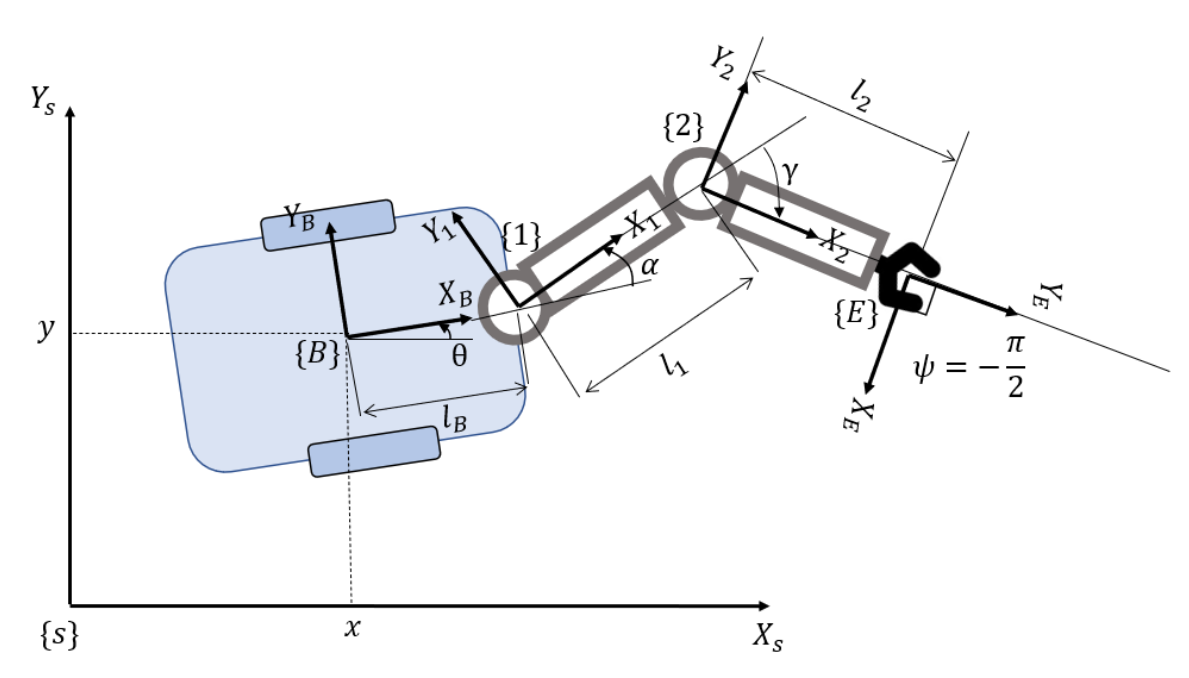
\includegraphics[width=0.7\textwidth]{img/mobile_manipulator.png}
    \caption{Mobile robot with plannar serial manipulator}
    \label{fig:Mobile Manipulator}
\end{figure}

\newpage
\section{Differential-Drive Simulation [25 pts]}
Create a simulation for the 2WD robot with \underline{Python} which takes as inputs the linear and angular velocities $\begin{bmatrix}
    v,\omega
\end{bmatrix}^\top$ (you can use the state space form). You should obtain the poses of the robot $\begin{bmatrix}
    x(t),y(t),\theta(t)
\end{bmatrix}^\top$ as outputs. 
\begin{enumerate}[(a)]
    \item Simulate and plot the trajectories obtained for the following velocities (use at least 30 seconds with a timestep of 0.1s):
    \begin{enumerate}[i.]
        \item Constant velocities
        \begin{enumerate} [1.]
            \item $\begin{bmatrix}
    v,\omega
\end{bmatrix}^\top=\begin{bmatrix}
    1,0
\end{bmatrix}^\top$
\item $\begin{bmatrix}
    v,\omega
\end{bmatrix}^\top=\begin{bmatrix}
    0,0.5
\end{bmatrix}^\top$
\item $\begin{bmatrix}
    v,\omega
\end{bmatrix}^\top=\begin{bmatrix}
    1,0.5
\end{bmatrix}^\top$
        \end{enumerate}
        \item Velocity profiles: $\begin{bmatrix}
            v(t)\\\omega(t)
        \end{bmatrix}=\begin{bmatrix}
            1+0.2\cdot\sin(t)\\
            0.2+0.6\cdot\cos(t)
        \end{bmatrix}$
    \end{enumerate}
    Linear velocities are [m/s] and angular velocities are [rad/s]. For each case, plot the top view of the 2D trajectory ($x$ vs $y$), and then each variable against time, including orientation $\theta$. Discuss briefly your observations on the outcome (feel free to perform more tests). [20 pts]
    \item 	Assuming the robot has dimensions $T$ (track) $= 0.3$ [m], and wheel radius $r = 0.15$ [m], what are the wheel speeds $u_l$,$u_r$ needed to achieve the constant velocities in (a).i? 
    
    Briefly comment on how you would need to change your implemented simulation if instead of linear and angular velocities, the input control parameters were wheel speeds. [5 pts]


\end{enumerate}
\section{3-Omniwheel Simulation [50 pts]}
\begin{enumerate}[(a)]
    \item Derive the equation of motion (as we did for the 4W during the lectures) for the omnidirectional wheeled robot with three wheels shown in see Figure~\ref{fig:3omni} [20 pts]
    
    \item Create a simulation for this robot with MATLAB or Python (you want to obtain $x,y,\theta$ for your simulation, you can obtain $\dot{x},\dot{y},\dot{\theta}$ as function of the wheels speeds by inverting the relationship obtained in (a)). Use $r=10$ cm and $l=25$ cm. [30 pts]
    \begin{enumerate}[I.]
        \item Apply rotation inputs (wheel rotation speeds) of $u_1=-2$ rad/s, $u_2=1.0$ rad/s and $u_3=1.0$ rad/s to the wheels and plot the true robot motion $(x,y,\theta)$ for 30 seconds. Plot the variables against time, and also a top view of the trajectory ($x$ vs $y$).
        \item Design control signals $(u_1,u_2,u_3)$ that will allow the robot to move in the following paths (simulation time is up to you, we recommend using at least 30 seconds):\begin{enumerate} [1)]
            \item a straight line with a slope of 60 degrees
            \item turn in a 2-meter diameter circle.
            \end{enumerate} 
        Use your simulation to confirm the obtained control signals by plotting the two cases, plot the variables against time, and also a top view of the trajectory ($x$ vs $y$). 
    \end{enumerate} 
\end{enumerate}
\begin{figure}[h!]
    \centering
    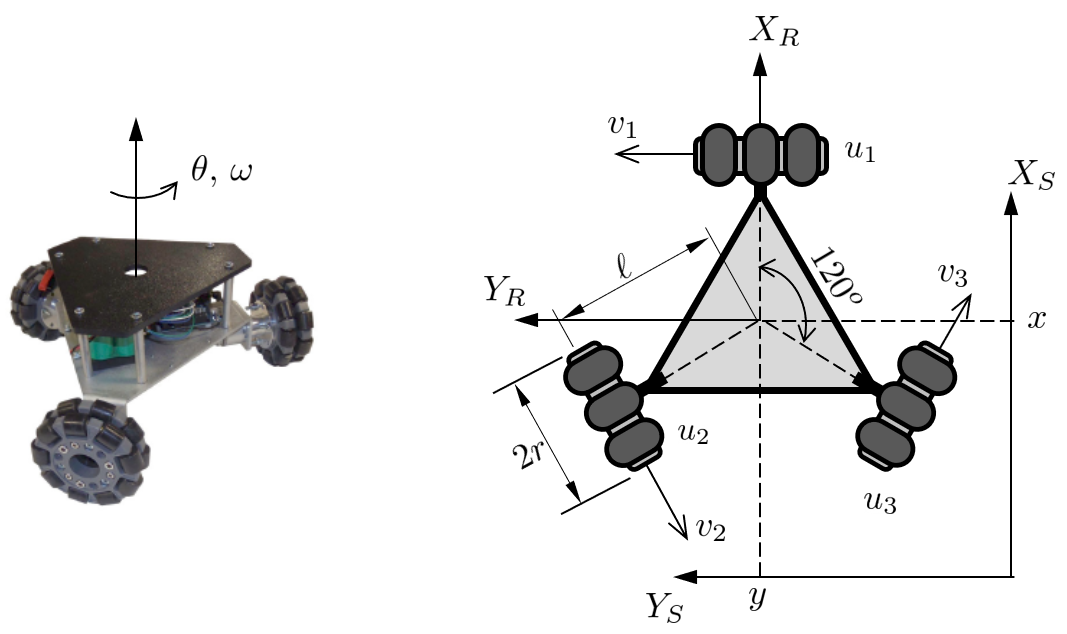
\includegraphics[width=0.7\textwidth]{img/omni.png}
    \caption{3W omnidirectional robot}
    \label{fig:3omni}
\end{figure}
%\input{problem_4}
\newpage

%%%%%%%%%%%%%%%%%%%%%%%%%%%%

\section*{Notes}

\begin{itemize}
    \item We are providing a Python example of how to code a simulation (see ``simulation\_example``). Ask TAs for help if you are facing difficulties with using MATLAB or Python for simulations.
    \item GenAI usage is allowed only to aid, but not generate, programming for all exercises. Students must retain a record of any GenAI interactions used in completing an exercise, including relevant prompts and responses. The instructing team reserves the right to request these records to verify compliance with the course's GenAI policy.
    \item Programming: for Matlab, use Livescript; if you use Python, deliver something that can be executed (e.g. Collab). Failing to submit an executable format that can be checked by the instructor will result in 0 points for the programming portion.
\end{itemize}


\section*{Submission Guideline}

Submit on LEARN Dropbox by October 2nd, 11:59PM. Late penalty applies as per syllabus if not properly justified. Overlaps with other assignments and/or course duties are not accepted as justifications. 

Answer each exercise thoroughly but concisely; computer-typed answers are preferred, especially for text. For equations, computer typed (MS Word/LaTex) is preferred, but hand-written ones are also accepted upon the condition that they are neat and readable. 

\quad

\noindent Files for submission:  

\begin{enumerate} [1.]
    \item One PDF report with all required answers and plots. All plots must have axes clearly labeled with units included, and a caption. Answers must be reported in the report and not only in the code.  
    \item One ZIP file containing:
    \begin{itemize}
        \item source code,
        \item scripts/notebooks,  
        \item helper files if needed.  
    \end{itemize}
\end{enumerate}
Include details of all analytical computations and assumptions made (if any) and required plots in your assignment report. There is no page limit. Code must be commented appropriately by yourself and not with GenAI.  

\end{document}